\documentclass[11pt, letterpaper]{elsarticle}
\usepackage{amsmath}
\usepackage{amssymb}
\usepackage{tikz}
\usepackage{tikz,fullpage}
\usepackage{pgf}
\usepackage{pgfplots}
\usetikzlibrary{
	pgfplots.fillbetween,
}
\usetikzlibrary{arrows,automata}
\usepackage{tkz-berge}

\begin{document}

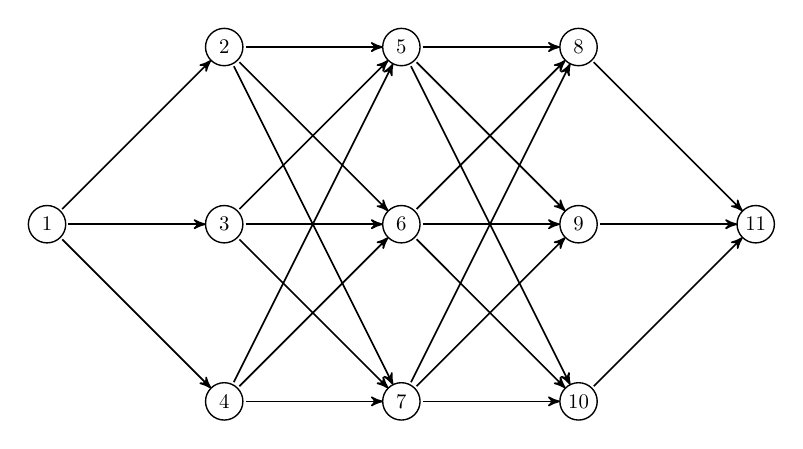
\begin{tikzpicture}[scale=0.75,transform shape]
	\Vertex[x=0,y=0]{1}
	\Vertex[x=3,y=3]{2}
	\Vertex[x=3,y=0]{3}
	\Vertex[x=3,y=-3]{4}
	\Vertex[x=6,y=3]{5}
	\Vertex[x=6,y=0]{6}
	\Vertex[x=6,y=-3]{7}
	\Vertex[x=9,y=3]{8}
	\Vertex[x=9,y=0]{9}
	\Vertex[x=9,y=-3]{10}
	\Vertex[x=12,y=0]{11}
	\tikzstyle{LabelStyle}=[fill=white,sloped]
	\tikzstyle{EdgeStyle}=[post]
	\Edge(1)(2)
	\Edge(1)(3)
	\Edge(1)(4)
	\Edge(8)(11)
	\Edge(9)(11)
	\Edge(10)(11)
	\Edge(2)(5)
	\Edge(2)(6)
	\Edge(2)(7)
	\Edge(3)(5)
	\Edge(3)(6)
	\Edge(3)(7)
	\Edge(4)(5)
	\Edge(4)(6)
	\Edge(4)(7)
	\Edge(5)(8)
	\Edge(5)(9)
	\Edge(5)(10)
	\Edge(6)(8)
	\Edge(6)(9)
	\Edge(6)(10)
	\Edge(7)(8)
	\Edge(7)(9)
	\Edge(7)(10)
	\end{tikzpicture}

\end{document}